\section{为什么长程对话记忆需要交互式评测}

\subsection{结论先行：记忆评测必须贴近真实部署}

长程对话中的 agent memory 评测，核心目标是判断一个真实参与对话的 assistant 是否能在长期交互中持续维护准确、可用、可更新的用户信息；一次离线阅读理解测试覆盖不了这个目标。讲者开场给出的 500 轮对话例子非常直接：用户在第 3 轮提到食物过敏，几百轮之后，assistant 仍然需要在后续建议中尊重这条关键信息。这个例子把 agent memory 从抽象指标拉回到真实使用场景：记忆成功意味着长期协作可以延续，记忆失败会带来前后矛盾、重复询问和信任损失。

本开场模块包含两个连续章节：第一章回答“为什么静态 benchmark 会低估真实部署风险”，第二章回答“为什么 AMemGym 要转向 on-policy 闭环”。两章共享同一条论证链：真实记忆能力来自 agent 参与形成的 interaction trajectory，因此评测也要保留 agent 回复对后续上下文的影响。

\begin{figure}[H]
    \centering
    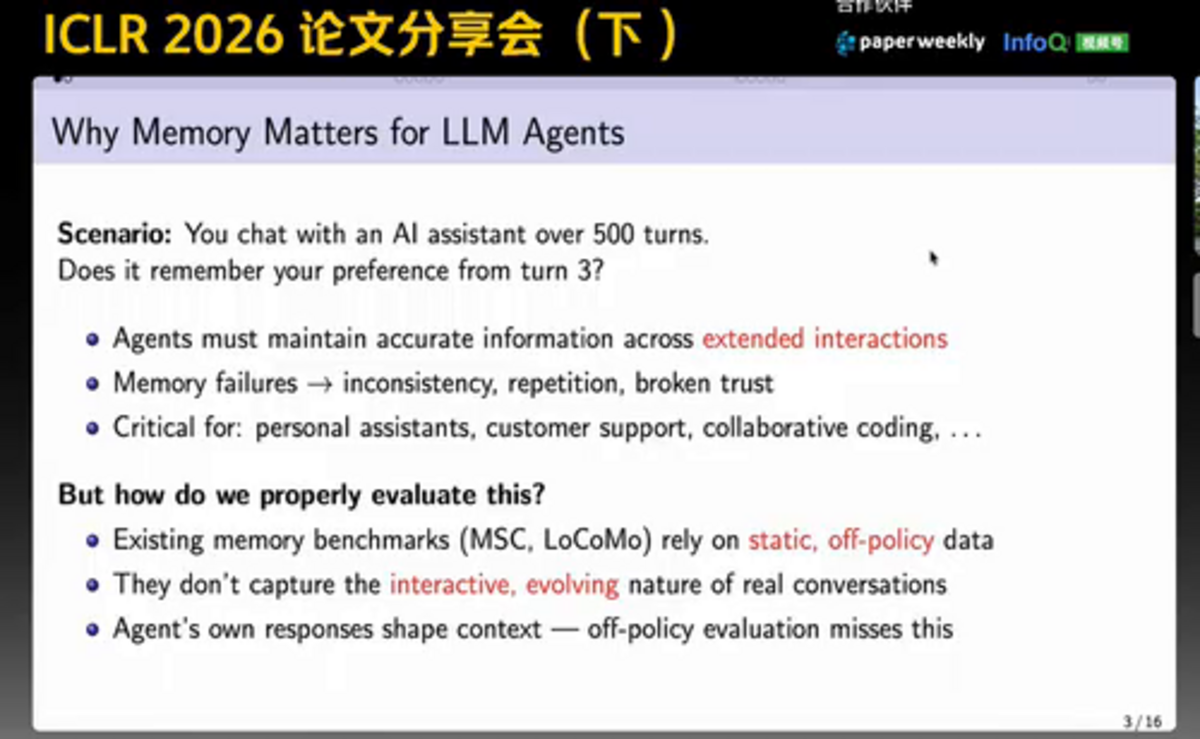
\includegraphics[width=0.82\linewidth,height=0.34\textheight,keepaspectratio]{figures/fig01_why_memory_matters.png}
    \caption[长程对话记忆的基本动机]{长程对话记忆的基本动机：assistant 需要跨越大量轮次维护准确用户信息，记忆失效会破坏一致性、效率和信任。\protect\footnotemark}
    \label{fig:why-memory-matters}
\end{figure}
\footnotetext{视频时间：00:00:40--00:01:40。}

图~\ref{fig:why-memory-matters} 的价值在于把“记忆”拆成了三个可观察后果。第一，assistant 需要在 extended interactions 中维持信息准确性；第二，记忆失败会表现为 inconsistency、repetition 与 broken trust；第三，这类能力在 personal assistant、customer support、collaborative coding 等长期任务中属于基础可靠性要求。换成直观类比，长期对话里的记忆像一份正在被共同编辑的项目笔记：若笔记丢了早期约束，后面的每一次建议都有可能偏离用户真实需求。

\begin{importantbox}{核心判断}
长程 agent memory 的评测对象应当是“参与交互后的记忆能力”。如果评测只让 agent 读取一段预写对话再答题，结果更接近对话阅读理解；真实部署里更关键的变量是 agent 自己的回复如何进入后续上下文，并继续影响未来要回忆的内容。
\end{importantbox}

\subsection{为什么静态 benchmark 会低估问题复杂度}

讲者指出，现有 memory benchmark 中的典型工作，如 MSC、LoCoMo 等，多数依赖 static、off-policy 的评估数据。这里的 `off-policy evaluation` 指一种离线评测设定：被测 agent 读取预先写好的 conversation，然后根据这段固定历史回答问题。这个设定便于构造数据集，也便于不同模型在同一材料上比较；它的代价同样清楚：agent 没有参与对话本身，自己的回复不会成为历史的一部分，评测过程缺少真实交互里的因果闭环。

在真实部署里，用户说出一个事实之后，assistant 的回答会影响下一步对话如何展开。比如 assistant 追问得更具体，用户可能补充更多细节；assistant 误解了用户，用户可能纠正或转移话题。静态 benchmark 固定了对话轨迹，使所有 agent 面对同一份历史材料，削弱了记忆机制对上下文生成过程的影响。

\begin{knowledgebox}{术语区分：static、off-policy、on-policy}
`static` 强调数据轨迹固定；`off-policy` 强调被测 agent 没有按照自己的策略生成这条轨迹；`on-policy` 强调 agent 实时参与交互，后续评测基于它亲自参与过的轨迹。三者可用自动驾驶类比理解：看别人已经录好的行车录像再回答路况问题，属于离线判断；车辆自己上路行驶，后续评估它在自己行动造成的路况中是否仍能安全决策，才接近闭环评测。
\end{knowledgebox}

\subsection{旧评测的两个关键缺口}

图~\ref{fig:existing-benchmarks} 对已有 benchmark 做了横向比较。表中已有方法的 Eval. Mode 一列均显示为 Static，Optimization Feedback 一列均没有给出正向标记；AMemGym 这一行则标为 Interactive，并带有 Optimization Feedback，同时自动化程度为 Fully Auto，对话长度为 Configurable。讲者据此归纳出两个缺口：评测模式停留在静态 off-policy；评测结果只能告诉开发者总体得分，难以指出记忆系统该在哪里改。

\begin{figure}[H]
    \centering
    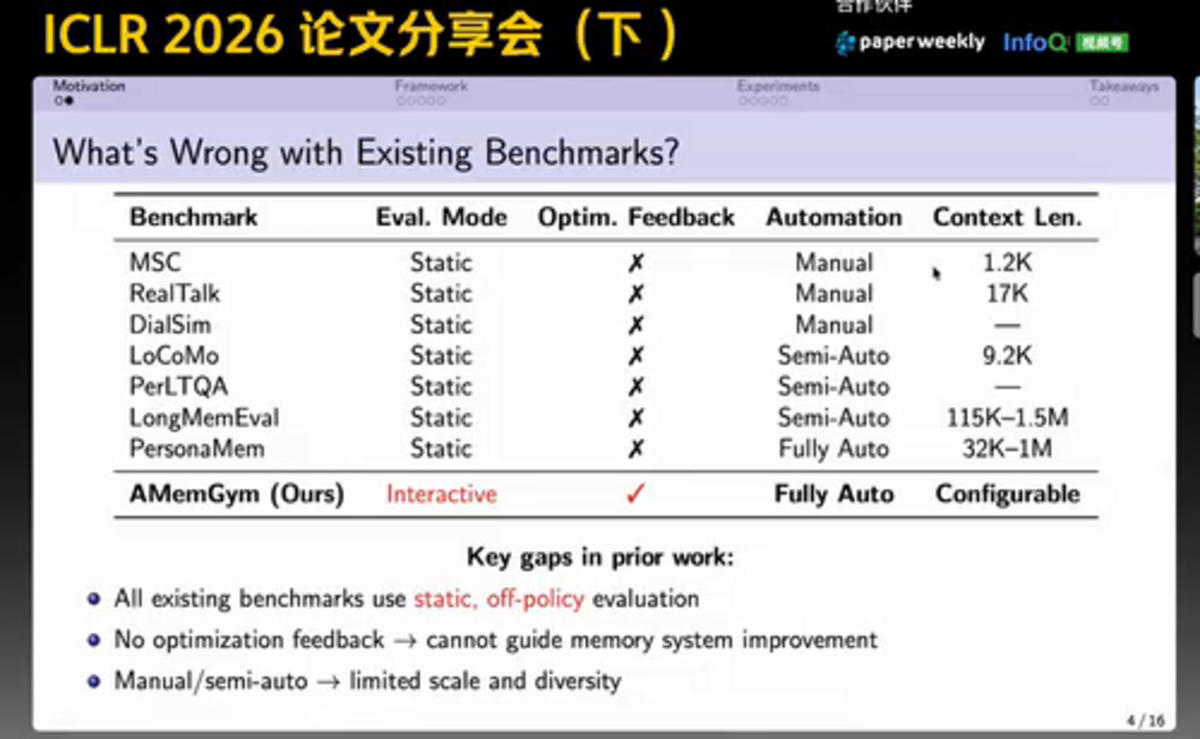
\includegraphics[width=0.82\linewidth,height=0.34\textheight,keepaspectratio]{figures/fig02_existing_benchmarks.png}
    \caption[已有长程记忆 benchmark 的对比]{已有长程记忆 benchmark 的对比：旧方法集中在 static、off-policy 设定，AMemGym 试图补上交互式评测和优化反馈。\protect\footnotemark}
    \label{fig:existing-benchmarks}
\end{figure}
\footnotetext{视频时间：00:02:40--00:04:20。}

第一个缺口是评测形态。若每个 agent 读取完全相同的预写对话，系统之间的区别会被压缩到“能否从文本中找回答案”这一层。这样的得分仍然有用，却难以代表长期 assistant 在真实环境中持续维护用户状态的能力。

第二个缺口是优化反馈。一个 overall score 可以告诉研发人员模型得了多少分，例如视频中用“60 分”作直观说明；它无法直接回答更重要的工程问题：失败来自写入、读取、利用，还是来自对更新信息的追踪。没有诊断指标时，团队容易进入盲目试错：换检索策略、换摘要策略、换上下文长度，每次都像在黑盒外面敲一敲，观察总分是否变化。

\begin{warningbox}{常见误解}
把长程对话记忆评测简化成“长上下文问答”会掩盖交互因素。长上下文问答关注给定文本中的信息检索；长程 agent memory 还涉及信息何时写入、旧信息何时更新、assistant 的回复如何改变下一轮用户输入，以及系统能否把记忆用于后续决策。
\end{warningbox}

\subsection{AMemGym 在这一章承担的角色}

AMemGym 的开场定位可以概括为两步。第一步，将 evaluation mode 从静态读取切换到交互式、动态的评估框架。第二步，在 overall metrics 之外加入 diagnostic metrics，让评测结果能反向指导记忆系统优化。讲者还提到该框架支持可配置的对话长度，并考虑数据多样性；这些细节为后续章节的 schema-based state evolution、checkpoint memory query 和 failure 分解埋下伏笔。

本章的术语校正和来源追踪作为写作脚注处理，正文继续保留概念主线。\footnote{本开场模块的关键来源区间：500 轮对话与食物过敏例子来自 00:00:40--00:01:40；benchmark 横向比较来自 00:02:40--00:04:20；瑜伽切换游泳与 off-policy/on-policy 路径对照来自 00:06:20--00:07:05。字幕里的 “MMGM / M m jm” 按封面和合同校正为 `AMemGym`；“of policy” 校正为 `off-policy`；“overall the matrix” 按上下文校正为 `overall metrics` 或 `diagnostic metrics`。这些校正只处理术语识别错误，未补写视频没有明确给出的模型名单、实验数值或论文公式。}

\subsection{本章小结}

本章的主线是：长程对话记忆影响真实部署中的信任，静态 off-policy benchmark 难以覆盖这种风险。500 轮对话与食物过敏的例子说明，agent memory 属于长期 assistant 的可靠性基础，不能被当成锦上添花的体验项。已有 benchmark 的主要问题集中在两处：评测轨迹固定，缺少优化反馈。AMemGym 因而把问题推进到交互式评测与诊断指标上：它关心 agent 如何在自己参与形成的上下文中记住、更新并使用信息。

\section{核心转向：闭环对话中的 on-policy 评测}

\subsection{结论先行：评测要保留“回复塑造上下文”的闭环}

第二章的核心转向是 `on-policy evaluation`：agent 需要实时参与对话，评测也要基于它亲自参与过的交互轨迹。原因很朴素：记忆机制会影响 agent 的回复，回复会进入后续上下文，后续上下文又决定未来的 memory query 到底在考什么。这个闭环一旦被切断，评测结果就会偏离真实部署。

可以把这件事理解成课堂讨论。教师想评估学生是否记住了前面同学提出的问题，如果只给学生一份别班讨论记录，再让他回答问题，测到的是读记录的能力；如果学生从头参与本班讨论，他的提问、误解和补充都会影响后续讨论内容，最终评估才更贴近真实互动。长程 assistant 也一样：它的每次回复都在共同写入未来上下文。

\subsection{瑜伽到游泳：同一事实如何分叉出不同轨迹}

讲者用一个具体例子解释这种耦合关系。用户在对话中说：“我上个月从练瑜伽切换成了游泳。”在 off-policy 设定下，Agent A 与 Agent B 都读取同一段预写 conversation；它们看到的上下文完全相同，因此差异主要体现在能否从固定文本中找回答案。

进入 on-policy 设定后，差异会被放大成不同对话轨迹。Agent A 记住用户喜欢运动，于是自然回应“好的，我换成游泳了”这类承接；Agent B 遗忘了之前的信息，转而提问“你之前有在做什么运动吗”。两种回复都会成为后续历史的一部分。Agent A 的历史里保留了对用户状态更新的承接；Agent B 的历史里出现了重复询问和信息断裂。之后再插入 memory query，两个 agent 面对的已经是由自己行为塑造出的不同上下文。

\begin{importantbox}{闭环评测的关键}
on-policy 评测保留三层耦合：记忆设计影响回复，回复改变对话轨迹，对话轨迹再影响后续记忆问题。AMemGym 要测试的正是这条链路；固定文本中的事实回忆只是其中一个较窄的子问题。
\end{importantbox}

\subsection{off-policy 与 on-policy 的路径差异}

图~\ref{fig:onpolicy-vs-offpolicy} 把路径差异压缩成左右对照。左侧 off-policy 路径中，dialogue generator 先生成 static history，然后不同 assistant 在同一历史上回答 recall question；右侧 on-policy 路径中，simulated user 与 assistant 共同生成 history A 或 history B，之后再基于对应轨迹发起回忆测试。图中的中心区别是“被测 agent 是否参与生成被评测的对话历史”。

\begin{figure}[H]
    \centering
    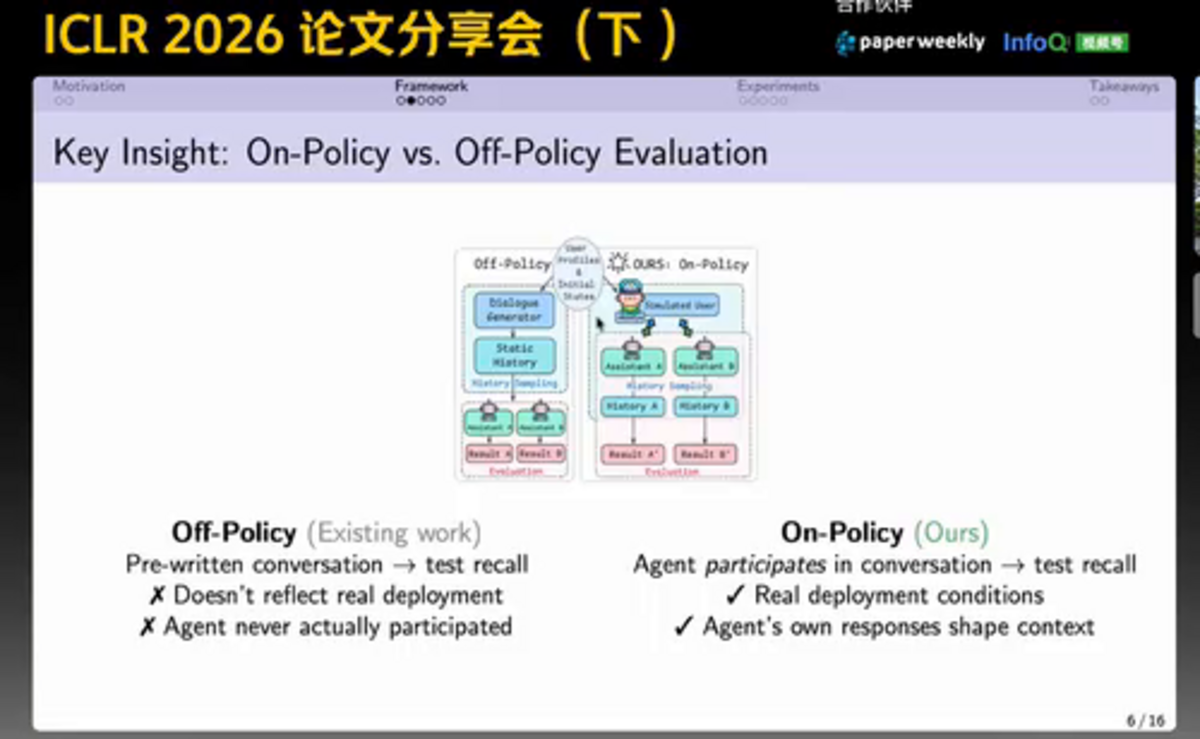
\includegraphics[width=0.82\linewidth,height=0.34\textheight,keepaspectratio]{figures/fig03_onpolicy_vs_offpolicy.png}
    \caption[off-policy 与 on-policy 的评测路径对照]{off-policy 与 on-policy 的评测路径对照：左侧使用预写对话测试 recall，右侧让 agent 参与生成自己的交互历史后再测试 recall。\protect\footnotemark}
    \label{fig:onpolicy-vs-offpolicy}
\end{figure}
\footnotetext{视频时间：00:06:20--00:07:05。}

从工程角度看，这个差异会影响结论可信度。off-policy 设定适合做固定材料上的横向比较，成本低、复现容易；on-policy 设定更接近 deployed assistant，因为 agent 的每次回复都可能引发用户补充、纠正或改变任务方向。AMemGym 选择后者，是为了让评测压力落在真实记忆系统必须处理的位置：长期状态维护、上下文自我污染、旧事实更新，以及后续问题对早期信息的追踪。

\begin{warningbox}{评测设计风险}
如果开发者只看 off-policy 得分，系统可能在固定历史问答中表现稳定，却在真实交互中积累错误。早期一次遗忘会改变后续用户输入，进而让未来的 memory query 建立在一条已经偏移的轨迹上；这种误差传播在静态评测里很难显形。
\end{warningbox}

\subsection{从评测模式到后续框架}

这一章完成了 AMemGym 的概念转向：长程记忆评测要从“读一段历史后答题”推进到“参与生成历史后接受检查”。后续框架将围绕这个转向展开：user simulator 负责推动对话和状态变化，checkpoint 负责注入 memory query，diagnostic metrics 负责把失败拆成更具体的环节。这样，评测就能同时回答两个问题：agent 是否记住了信息，以及记忆系统在哪个环节让信息失真、丢失或无法被利用。

\begin{knowledgebox}{为什么 on-policy 更适合优化记忆系统}
记忆系统优化需要观察“策略改变以后会生成什么样的对话”。如果改进写入策略会让 assistant 更早确认用户偏好，后续上下文也会跟着改变；如果读取策略失误，assistant 可能不断重复询问，造成历史污染。on-policy 评测保留这种反馈回路，因此更适合诊断和迭代 memory system。
\end{knowledgebox}

\subsection{本章小结}

本章说明了 AMemGym 从 off-policy 走向 on-policy 的理由：agent memory 与对话轨迹彼此耦合。瑜伽切换游泳的例子显示，同一用户事实在不同记忆机制下会产生不同回复，进而形成不同历史。off-policy 评测固定历史，适合控制变量；on-policy 评测让 agent 参与生成历史，更贴近真实部署条件。这个转向为后续三阶段框架奠定基础：先生成可控状态，再进行闭环交互，最后用 memory query 与 diagnostic metrics 做细粒度评估。
